\chapter{A risk figure is an estimate}\label{ch:estimate}

A committee that has declared its adversary, as Chapter~\ref{ch:scenario} asks, and
settled which experiment its figure describes, as Chapter~\ref{ch:measures} asks, still
has to obtain the figure. For any realistic adversary the figure has no closed form. It
comes from simulating the attack many times and counting how often it succeeds. Most
committees then apply a rule that seems too plain to question: if the estimated risk is
below the tolerance, the release is safe enough to make.

The rule has a strong case. A simulated success rate is an unbiased estimate of the
risk it targets. Its standard error falls with the square root of the number of
simulated attacks, so a few thousand replicates give an estimate whose error is a small
fraction of any tolerance a committee is likely to set. The tolerance itself is a
judgement, often rounded to one significant figure, and set beside that judgement the
second decimal place of a well-run simulation can seem beside the point. On this view the
estimate is the best single guess at the risk, and a decision based on the best guess is
the reasonable one.

The fact that breaks the rule concerns the releases it is meant to stop. Take a release
whose true risk sits exactly at a tolerance of 0.12 and estimate that risk from 1,200
independent simulated attacks, the replicate count of the simulation study. The
estimate falls at or below the tolerance with probability 0.52.
% computed from the Binomial(1200, 0.12) distribution: P(X <= 144) = 0.522; B = 1,200 from paper/bis_ifc_full.tex line 3480 and tau = 0.12 from line 832
At the boundary the rule is a coin toss, and it stays close to one for releases a little
above the boundary: at a true risk of 0.125 it still releases about one time in three.
% computed: P(X <= 144 | Binomial(1200, 0.125)) = 0.319
A committee using it believes that it keeps risk below the tolerance. What it keeps
below the tolerance is a random number whose mean is the risk, and the decision record,
which holds only that number, cannot show the difference.

The chapter asks one question. How much evidence must a simulated risk figure carry
before a committee may conclude that the risk lies at or below its tolerance?

\section{A figure just under the line}

The question reached the Bank in a committee meeting. Naledi had assessed a household
survey release with age in twenty-year bands, three occupation groups and a minimum cell
count of ten. Against the stronger of the two declared adversaries her simulation named
the target in 127 of 1,200 attacks, a rate of 0.1058, and the committee's tolerance was
0.12.
% source: artifacts-paper/results.json (grid.settings, "20-year bands, 3 groups, k_min = 10": risk = 0.10583, replicates = 1200); paper/bis_ifc_full.tex lines 832-834
The chair read the figure, saw that it was below the line, and asked whether anyone
objected to release.

Naledi did. Her paper carried a second column, an upper confidence bound at the 95 per
cent level, and in that column the same setting stood at 0.1216, above the tolerance.
% source: artifacts-paper/results.json (risk_upper = 0.12158); paper/bis_ifc_full.tex line 834
She recommended that the committee not release on this evidence. The chair's reply was
the natural one: the best estimate of the risk was below the tolerance, so on what
grounds should a second, larger number decide? The rest of this chapter is the answer
Naledi gave.

\section{The estimate and its error}

Let the declared attack be simulated $B$ times under the declared scenario, each
replicate drawing a target and the adversary's information afresh, and let
$C^{(b)} = 1$ if replicate $b$ names the target correctly. The Monte Carlo estimator of
the risk $R$ is the success rate,
\begin{equation}\label{c04:eq-mc}
\widehat{R} = \frac{1}{B}\sum_{b=1}^{B} C^{(b)}, \qquad
\E[\widehat{R}] = R, \qquad
\mathrm{Var}(\widehat{R}) = \frac{R(1-R)}{B}.
\end{equation}
The variance formula holds because the $C^{(b)}$ are independent Bernoulli variables
with success probability $R$, and $X = B\widehat{R}$ is then binomial. Both facts
depend on how the simulation was built. If the replicates share an auxiliary file, a
set of released records or a fitted model, they are not independent, and
\eqref{c04:eq-mc} understates the variance. The cure is to resample the unit that is
shared, the auxiliary file or the fitted parameters, and recompute the risk within each
resampled unit \citep{efron1993}, so that the spread between units carries the
dependence. Section~\ref{c04:sec-layers} returns to this as an analysis of variance. For
now take the replicates to be independent, which in the simulation study they are,
conditional on the realised sample and mechanism output.

The estimate is unbiased, and its standard error at the Bank's figure is 0.0089, the
square root of $0.1058 \times 0.8942 / 1200$.
% arithmetic from the values above
That is less than a tenth of the tolerance, which is the source of the chair's
confidence. The gap between the estimate and the tolerance, 0.014, is less than two
standard errors, and that is the source of Naledi's doubt.

\section{What a point-estimate rule does at the boundary}

The behaviour of a decision rule is best read from its operating characteristic, the
probability that it releases as a function of the true risk. Figure~\ref{c04:fig-oc}
plots it for two rules at $B = 1{,}200$ and a tolerance of 0.12. The solid line is the
rule that releases when $\widehat{R} \le \tau$. The dashed line is the rule that releases
when an exact one-sided 95 per cent upper bound is at or below $\tau$, the rule defined
in the next section.

\begin{figure}[t]
\centering
% Computed exactly from the binomial distribution with B = 1,200 and tau = 0.12
% (point rule: release iff X <= 144; bound rule: release iff X <= 125, the largest count
% whose Clopper--Pearson 95 per cent upper bound is at most 0.12). These curves are a
% calculation from the formulas of this chapter, not an output stored in the repository.
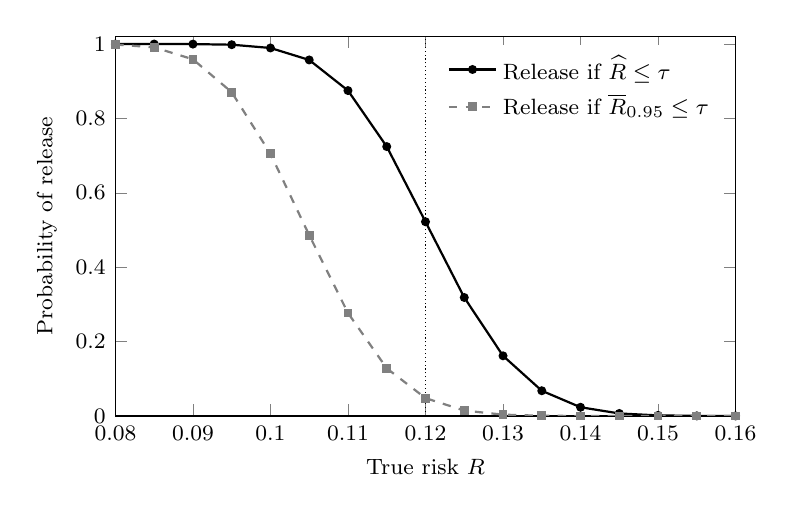
\begin{tikzpicture}
\begin{axis}[width=0.78\textwidth, height=6.4cm,
  xmin=0.08, xmax=0.16, ymin=0, ymax=1.02,
  xlabel={True risk $R$}, ylabel={Probability of release},
  xtick={0.08,0.09,0.10,0.11,0.12,0.13,0.14,0.15,0.16},
  xticklabel style={/pgf/number format/fixed, /pgf/number format/precision=2},
  label style={font=\footnotesize}, tick label style={font=\footnotesize},
  legend style={font=\footnotesize, at={(0.98,0.98)}, anchor=north east, draw=none},
  legend cell align=left]
\addplot[black, thick, solid, mark=*, mark size=1.2pt] coordinates {
 (0.080,1.0000) (0.085,1.0000) (0.090,0.9998) (0.095,0.9982) (0.100,0.9894)
 (0.105,0.9572) (0.110,0.8749) (0.115,0.7243) (0.120,0.5222) (0.125,0.3186)
 (0.130,0.1618) (0.135,0.0679) (0.140,0.0235) (0.145,0.0068) (0.150,0.0016)
 (0.155,0.0003) (0.160,0.0001)};
\addlegendentry{Release if $\widehat{R} \le \tau$}
\addplot[gray, thick, dashed, mark=square*, mark size=1.2pt, mark options={solid}] coordinates {
 (0.080,0.9987) (0.085,0.9911) (0.090,0.9589) (0.095,0.8705) (0.100,0.7049)
 (0.105,0.4862) (0.110,0.2769) (0.115,0.1282) (0.120,0.0481) (0.125,0.0146)
 (0.130,0.0036) (0.135,0.0007) (0.140,0.0001) (0.145,0.0000) (0.150,0.0000)
 (0.155,0.0000) (0.160,0.0000)};
\addlegendentry{Release if $\overline{R}_{0.95} \le \tau$}
\draw[densely dotted] (axis cs:0.12,0) -- (axis cs:0.12,1.02);
\end{axis}
\end{tikzpicture}
\caption{Probability that each rule releases, against the true risk, with $B = 1{,}200$
independent simulated attacks and a tolerance $\tau = 0.12$ (dotted line). The rules are
told apart by line style, shade and marker. At $R = \tau$ the point-estimate rule
releases with probability 0.52 and the bound rule with probability 0.048. Exact binomial
calculation.}
\label{c04:fig-oc}
\end{figure}

The solid curve crosses one half at the tolerance. That is the general pattern, and it
holds for any estimator that is centred on the truth.

\begin{proposition}[A point estimate at the tolerance]\label{c04:prop-point}
Suppose a rule releases whenever $\widehat{R}_B \le \tau$, where $\widehat{R}_B$ is
a consistent estimator of $R$ with $\sqrt{B}(\widehat{R}_B - R)$ converging in law to
a distribution symmetric about zero and continuous at zero. If $R = \tau$, the rule
releases with probability tending to $1/2$ as $B \to \infty$. If instead the rule
releases only when a one-sided upper bound $\overline{R}_{1-\alpha}$ with
$\Prob\{\overline{R}_{1-\alpha} \ge R\} \ge 1-\alpha$ is at or below $\tau$, then for
every $R > \tau$ the rule releases with probability at most $\alpha$.
\end{proposition}

The proposition does not say that point estimates are poor estimates. It says that a
rule which compares a point estimate with a line has no control over the error it
exists to prevent. More replicates sharpen the solid curve in Figure~\ref{c04:fig-oc}
towards a step at $\tau$, but they do not move the half at $\tau$ itself, and the
releases near the line are the ones a committee most needs its rule to handle. The
bound rule fixes the chance of a wrong release for every risk above the tolerance at
$\alpha$ or less, and the dashed curve shows the price: it releases less often below
the line. Section~\ref{c04:sec-suppression} weighs that price.

Grace, reading the Bank's archive for the audit of Chapter~\ref{ch:measures}, met the
consequence in its plainest form. The past decision records held point estimates only,
some of them a few thousandths below their tolerances. For each such record she could
see that the committee had released, and she could not tell whether the release had been
a sound one or the lucky side of a coin. The record did not hold the number of
replicates, so the uncertainty could not be rebuilt. Her finding recommended that every
risk figure in a decision record carry its replicate count and its bound.

\section{Exact one-sided bounds}

The bound rule needs a bound that is valid at the risks the committee faces, which are often
small. The normal approximation, $\widehat{R} + z_{1-\alpha}\sqrt{\widehat{R}(1-\widehat{R})/B}$,
is unreliable there: its coverage falls short of the nominal level for small $R$ and
moderate $B$, and it collapses to zero when no attack succeeds \citep{brown2001}. The
exact bound of \citet{clopper1934} has no such failure. If $X = x$ of $B$ independent
attacks succeed, the one-sided $(1-\alpha)$ upper bound is
\begin{equation}\label{c04:eq-cp}
\overline{R}_{1-\alpha}(x,B) = \mathrm{Beta}^{-1}_{1-\alpha}(x+1,\,B-x), \qquad x < B,
\end{equation}
and one when $x = B$, where $\mathrm{Beta}^{-1}_{q}(a,b)$ is the $q$th quantile of a
beta distribution. Equivalently, $\overline{R}_{1-\alpha}(x,B)$ is the risk at which the
chance of seeing $x$ or fewer successes is exactly $\alpha$: a larger risk would make the
observed count implausibly low.

\begin{proposition}[Validity of the exact bound]\label{c04:prop-cp}
If $X \sim \mathrm{Binomial}(B,R)$, then
$\Prob_R\{\overline{R}_{1-\alpha}(X,B) < R\} \le \alpha$ for every $R \in [0,1]$.
\end{proposition}

\begin{example}[Naledi's 127 successes]\label{c04:ex-naledi}
The attack named the target in $x = 127$ of $B = 1{,}200$ attacks, so
$\widehat{R} = 127/1200 = 0.1058$. Its standard error is
$\sqrt{0.1058 \times 0.8942/1200} = 0.0089$. The normal approximation gives an upper
bound of $0.1058 + 1.645 \times 0.0089 = 0.1204$. The exact bound
\eqref{c04:eq-cp} is the 0.95 quantile of the $\mathrm{Beta}(128, 1073)$ distribution,
which is $0.1216$. Both lie above the tolerance of 0.12, the exact one by a little more.
At this number of attacks the largest count of successes whose exact bound is at or
below 0.12 is 125, so the setting would have passed with two fewer successes and fails
with 127.
\end{example}

\begin{example}[A file that passes]\label{c04:ex-pass}
The worked example of the long-form paper shows the bound in use. On the confirmation
draw for the single-release attack on the synthetic credit register, the attack named
the right loan for 337 of 4,000 targets, a rate of 0.084. The 0.95 quantile of the
$\mathrm{Beta}(338, 3663)$ distribution is 0.092, below the tolerance of 0.12 with a
margin of 23 per cent of the tolerance, so the file passes for that adversary.
% source: paper/worked_examples.tex, Example ex:bound (337 of 4,000; 0.084; 0.092; margin 0.23)
The decision rests on the bound and not the rate. Had 458 of the 4,000 attacks succeeded, a rate of 0.115, the bound would have been
0.123, and the release would have failed.
\end{example}
% source: paper/worked_examples.tex, Example ex:bound and ex:selection (0.115, 0.123)

The case of no successes deserves its own formula, because it is the case a committee
with a small tolerance hopes to see. With $x = 0$ the beta quantile has a closed form,
since $\Prob_U(X = 0) = (1-U)^B$, and setting that to $\alpha$ gives
\begin{equation}\label{c04:eq-cp0}
\overline{R}_{1-\alpha}(0,B) = 1 - \alpha^{1/B} \approx \frac{-\log\alpha}{B}.
\end{equation}
At $\alpha = 0.05$, $-\log\alpha$ is close to three, which is the rule of three that
\citet{hanley1983} set out for clinical work: if none of $B$ patients suffers an adverse
event, the event rate may still be as high as about $3/B$. The same arithmetic applies
to an attack that never succeeds. No number of failed attacks shows that the risk is
zero. What a run of failures shows is an upper bound, and its strength is set by $B$
and nothing else.

\section{The price of a small tolerance}

Equation~\eqref{c04:eq-cp0} turns a tolerance into a budget. A committee that wants its
bound at or below $\tau$ from a run with no successes needs enough attacks to push
$1 - \alpha^{1/B}$ under $\tau$.

\begin{proposition}[Certification cost]\label{c04:prop-cert}
Suppose $B$ independent simulated attacks produce no success. The exact one-sided
$(1-\alpha)$ bound satisfies $\overline{R}_{1-\alpha} \le \tau$ if and only if
\begin{equation}\label{c04:eq-cert}
B \ \ge\ \frac{\log\alpha}{\log(1-\tau)},
\end{equation}
and the right side equals $-\log(\alpha)/\tau + O(1)$ as $\tau \downarrow 0$.
\end{proposition}

The cost grows in inverse proportion to the tolerance. Figure~\ref{c04:fig-cost} plots
the required number of attacks at five tolerances and two error levels. Certifying a
tolerance of 0.01 at $\alpha = 0.05$ takes 299 independent attacks with no success. A
tolerance of one in a thousand takes 2,995, and one in a hundred thousand takes 299,572;
at $\alpha = 0.01$ the last becomes 460,515.
% source: paper/generated/table_certification.tex
At the other end, a tolerance of 0.05 needs only 59 attacks, and the long-form paper's
worked example puts the figure for the credit register's tolerance of 0.12 at 24.
% source: paper/generated/table_certification.tex (59); paper/worked_examples.tex, Example ex:zero (24)
These counts are lower limits. They assume that every attack fails. If some succeed,
more are needed, and inverting \eqref{c04:eq-cp} for the observed count gives the number.

\begin{example}[Twenty-four clean attacks]\label{c04:ex-24}
For the credit register's tolerance of $\tau = 0.12$ at $\alpha = 0.05$,
\eqref{c04:eq-cert} asks for $B \ge \log 0.05/\log 0.88 = 23.4$, so 24 attacks. With 24
attacks and no success the bound is $1 - 0.05^{1/24} = 0.117$, which passes. With 23 the
bound is $0.122$, which fails. A single success among the 24 lifts the bound to $0.183$,
and the committee would then need many more attacks, not one more. The rule of three
gives $3/24 = 0.125$, close to the exact $0.117$ and on the safe side.
\end{example}

The practical content is that a tolerance and an evidence standard are one decision. A
committee that writes a tolerance of one in a hundred thousand into its policy has
committed itself to run several hundred thousand independent attacks for every release,
and to run them so that they really are independent, or else to replace simulation with
an argument from a model. If it cannot do either, the tolerance is not supported by its
evidence, and the decision record should say so. Choosing a small tolerance because it
sounds prudent, without pricing the evidence, produces a rule that no release can pass
on the evidence.

\begin{figure}[t]
\centering
% source: paper/generated/table_certification.tex (all ten points)
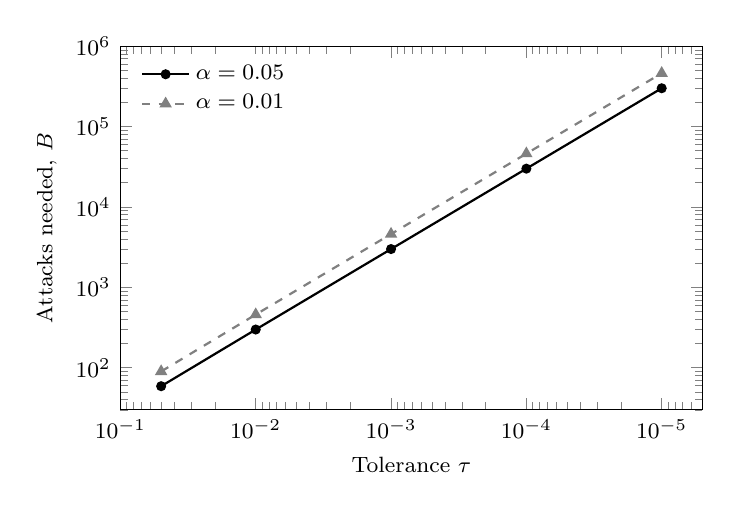
\begin{tikzpicture}
\begin{axis}[width=0.74\textwidth, height=6.2cm,
  xmode=log, ymode=log, x dir=reverse,
  xmin=5e-6, xmax=0.1, ymin=30, ymax=1e6,
  xlabel={Tolerance $\tau$}, ylabel={Attacks needed, $B$},
  label style={font=\footnotesize}, tick label style={font=\footnotesize},
  legend style={font=\footnotesize, at={(0.02,0.98)}, anchor=north west, draw=none},
  legend cell align=left]
\addplot[black, thick, solid, mark=*, mark size=1.4pt] coordinates {
 (0.05,59) (0.01,299) (0.001,2995) (0.0001,29956) (0.00001,299572)};
\addlegendentry{$\alpha = 0.05$}
\addplot[gray, thick, dashed, mark=triangle*, mark size=1.8pt, mark options={solid}] coordinates {
 (0.05,90) (0.01,459) (0.001,4603) (0.0001,46050) (0.00001,460515)};
\addlegendentry{$\alpha = 0.01$}
\end{axis}
\end{tikzpicture}
\caption{Independent simulated attacks, all failing, needed for the exact one-sided bound
to reach the tolerance, from Proposition~\ref{c04:prop-cert}. Both axes are logarithmic
and the tolerance falls from left to right. The error levels are told apart by line
style, shade and marker. Ten times smaller a tolerance costs ten times as many attacks.}
\label{c04:fig-cost}
\end{figure}

The practical content is that a tolerance and an evidence standard are one decision. A
committee that writes a tolerance of one in a hundred thousand into its policy has
committed itself to run several hundred thousand independent attacks for every release,
and to run them so that they really are independent, or else to replace simulation with
an argument from a model. If it cannot do either, the tolerance is not supported by its
evidence, and the decision record should say so. Choosing a small tolerance because it
sounds prudent, without pricing the evidence, produces a rule that no release can pass
on the evidence.

The published record of attacks offers no shortcut. A systematic review of
re-identification attacks on health data \citep{elemam2011} found that most were small,
and that most targeted data which had not been de-identified to any standard. It is
tempting to read such a record as evidence that properly protected data are rarely
re-identified. The record does not support that reading in the terms of this section. It
is not a count of independent attempts against protected releases, so it does not supply
the $B$ of \eqref{c04:eq-cp0}, and an absence of reported successes is not a run of
observed failures.

\section{The cost of the other error}\label{c04:sec-suppression}

The bound rule controls one error and leaves the other to the sample size. As in the
testing framework of \citet{neyman1933}, it fixes the more serious error, release
when the risk exceeds the tolerance, at a stated level. The other error is suppression
of a release whose true risk is below the tolerance, and Figure~\ref{c04:fig-oc} shows
how large it can be. At a true risk of 0.105, well inside the tolerance, the bound rule
with 1,200 attacks releases less than half the time.
% computed: P(X <= 125 | Binomial(1200, 0.105)) = 0.486 (same calculation as the figure)
The Bank's setting, with an estimate of 0.1058, sits in exactly that region.

The remedy is more attacks, and the calculation is short. The bound exceeds
the estimate by roughly $z_{1-\alpha}$ standard errors, about $1.645 \times 0.0089 =
0.015$ at the Bank's figure, and that margin shrinks with $\sqrt{B}$. If the true risk is
near 0.106, a margin of 0.014 between risk and tolerance needs the standard error to fall
below about 0.0085 for the bound to clear the line half the time, and well below it for
the bound to clear the line reliably.
% arithmetic: sqrt(0.1058*0.8942/1200) = 0.0089; 0.12 - 0.106 = 0.014; 0.014/1.645 = 0.0085
Four times the attacks halves the standard error. A committee that sees an estimate below
its tolerance and a bound above it has learned that the evidence is too thin to decide,
and the right response is to buy more evidence, not to choose the number that agrees with
the hoped-for answer.

That was Naledi's recommendation. The chair accepted that the committee could not
release on 1,200 attacks, and asked how many would settle the matter. Naledi's answer was that the count depended on where the true risk lay, which was the
thing being estimated. If it was near the estimate, about 5,000 attacks would put the
bound below 0.12 in nineteen runs of twenty.
% arithmetic: need (1.645 + 1.645) * sqrt(0.106 * 0.894 / B) <= 0.014, so B >= 5,200 approximately
If it was nearer the tolerance, no affordable number would,
and the committee would then be choosing between a stricter setting and a different
access route. Chapter~6 shows how to run the attacks in stages and stop as soon as the
evidence is sufficient, which an analyst may not do with the fixed-sample bound of this
chapter.

\section{Where the variance comes from}\label{c04:sec-layers}

The binomial variance in \eqref{c04:eq-mc} describes one source of error, the
simulation, and it describes it conditional on everything the simulation holds fixed.
A risk estimate has at least two further sources: the confidential sample, which is one
draw from the sampling design, and any parameters the adversary's model fits from an
auxiliary source. Writing $\mathcal{D}$ for the realised sample and $\widehat\eta$ for
the fitted inputs, the law of total variance separates the two kinds:
\begin{equation}\label{c04:eq-total}
\mathrm{Var}(\widehat R)
= \underbrace{\E\{\mathrm{Var}(\widehat R \mid \mathcal{D},\widehat\eta)\}}_{V_{\mathrm{MC}}}
 + \underbrace{\mathrm{Var}\{\E(\widehat R \mid \mathcal{D},\widehat\eta)\}}_{V_{\mathrm{input}}}.
\end{equation}
The binomial expression estimates only $V_{\mathrm{MC}}$. Increasing $B$ drives that term
towards zero and leaves $V_{\mathrm{input}}$ untouched. An interval built from
\eqref{c04:eq-mc} alone can therefore become as narrow as the analyst's computing budget
allows while the uncertainty that the institution actually faces stays where it was.

A nested design measures both terms. Draw outer replicates $s = 1, \dots, S$; in each,
redraw the confidential sample according to its design, refit any auxiliary model, apply
the mechanism and run $B$ attacks, giving an estimate $\widehat R_s$. With
$\overline{R} = S^{-1}\sum_s\widehat R_s$, the analysis of variance is
\begin{equation}\label{c04:eq-nested}
\widehat V_{\mathrm{within}} = \frac{1}{S}\sum_{s=1}^{S}\frac{\widehat R_s(1-\widehat R_s)}{B},
\qquad
\widehat V_{\mathrm{between}} = \frac{1}{S-1}\sum_{s=1}^{S}(\widehat R_s - \overline R)^2
 - \widehat V_{\mathrm{within}},
\end{equation}
with the second truncated at zero when it falls slightly negative.

\begin{proposition}[What the nested estimator estimates]\label{c04:prop-nested}
Let the outer replicates be independent, let $R_s$ be the risk conditional on the
sample and inputs of replicate $s$, and let $B\widehat R_s \mid R_s \sim
\mathrm{Binomial}(B,R_s)$. Write $V_{\mathrm{MC}} = \E[R_s(1-R_s)]/B$ and
$V_{\mathrm{input}} = \mathrm{Var}(R_s)$. Then
\begin{equation}\label{c04:eq-nested-exp}
\E\big[\widehat V_{\mathrm{within}}\big] = \frac{B-1}{B}\,V_{\mathrm{MC}},
\qquad
\E\Big[\frac{1}{S-1}\sum_{s}(\widehat R_s-\overline R)^2\Big] = V_{\mathrm{input}} + V_{\mathrm{MC}},
\end{equation}
so that, before truncation, $\E[\widehat V_{\mathrm{between}}] = V_{\mathrm{input}} +
V_{\mathrm{MC}}/B$.
\end{proposition}

The bias terms are of order $1/B$ and negligible at any useful replicate count, so the
two estimators split the variance as \eqref{c04:eq-total} does. The simulation study ran
this design on one setting of its grid, the same twenty-year, three-group, minimum ten
setting as the Bank's example above: 120 outer replicates, each redrawing the 5 per cent
sample from the same population and running 500 attacks.
% source: paper/generated/numbers.tex (\runnestedouter); artifacts-paper/results.json (design_variance: inner_replicates = 500, mechanism "20-year bands, 3 groups, k_min = 10")
The within-replicate standard deviation was 0.0112. The between-replicate standard
deviation came out at zero after the correction, and the standard error of the overall
mean was 0.0010 whether the design term was included or not.
% source: paper/generated/numbers.tex (\runnestedwithinsd, \runnestedbetweensd, \runnestedse, \runnestednaivese)
On this design, with 120 outer replicates, the sampling term was not detectable at that number of replicates.

The result does not license ignoring the design, and the reason is in its interval. A
chi-square interval for the total variance, carried through to the share of variance
that the design contributes, runs from 0 to 0.19.
% source: paper/generated/numbers.tex (\runnestedsharehigh = 19); artifacts-paper/results.json (between_share_interval = [0, 0.192])
The data would not have distinguished a design contribution of up to a fifth of the
variance from none. That interval assumes the outer estimates are roughly normal, which at 500 attacks and
a risk near 0.07 is reasonable, though it would not be for a risk near zero.
% source: artifacts-paper/results.json (design_variance.mean = 0.0674)
Three features of the synthetic design kept the term small: the population was large and
fixed, the sampling fraction was modest, and the adversary's model was not refitted
between replicates. None of them is guaranteed at an institution. In particular, an
institution that reuses one auxiliary file across all its replicates has made the
auxiliary file a shared unit, and \eqref{c04:eq-total} then has a third term that
\eqref{c04:eq-mc} cannot see. An analyst who reports a very tight interval from a very large $B$ should say which term
the large $B$ drove down.

Grace put this point to Naledi as a question about the Bank's own practice. The earlier
assessments had used one extract of the business register as the adversary's auxiliary
file for every replicate, so every simulated attack had drawn on the same file. Naledi
confirmed it, and agreed that the binomial bounds in those records described the
simulation and not the file. The new procedure resampled the auxiliary file within the
nested design, and the record stated which variance the reported bound covered.

\section{The worst target}

The risk in the preceding sections is an average over a target drawn from a declared
population. Rule \eqref{c04:eq-admiss} below is stated for a set $T$ of targets, as
Chapter~\ref{ch:decision} introduced it, and the set has to be explicit: a maximum over released
records, a maximum over a protected subgroup and an average over a population are three
controls, and a release can pass one and fail another. A release is statistically
admissible only if
\begin{equation}\label{c04:eq-admiss}
\sup_{t \in T}\ \overline{R}_{1-\alpha}(t,\theta) \ \le\ \tau .
\end{equation}

When $T$ is finite, the rule asks every target's bound to meet the tolerance. That is an
intersection--union test in the sense of \citet{berger1982}, and it needs no correction
for the number of targets.

\begin{proposition}[Every target must pass, at level $\alpha$ each]\label{c04:prop-iut}
Let $T$ be a finite set of targets, and for each $t \in T$ let $\overline{R}_t$ be a
one-sided bound with $\Prob\{\overline{R}_t < R_t\} \le \alpha$. The rule that releases
when $\overline{R}_t \le \tau$ for every $t \in T$ releases with probability at most
$\alpha$ whenever some target has $R_t > \tau$, whatever the dependence among the bounds.
\end{proposition}

The worst target raises a different question when the committee wants to report it. On
the synthetic register the long-form paper examined the targets in the smallest released
cells under minimum cell counts from 3 to 20, attacking each target 250 times. At a
minimum count of ten, 230 targets were examined, and the worst had an estimated risk of
0.744 against a nominal $1/k$ of 0.1.
% source: paper/generated/table_kanonymity.tex (k_min = 10: 230 targets, worst 0.744, 1/k = 0.1000)
That figure is selected: it is the largest of 230 estimates, and the largest of many
noisy estimates is biased upwards. A lower bound computed for that target as if it had
been chosen in advance would inherit the bias. The correction is to take each target's
lower bound at level $\alpha/q$ for $q$ examined targets, which makes the statement hold
for all targets at once.

\begin{proposition}[A lower bound for the selected worst target]\label{c04:prop-selmax}
Let $T$ hold $q$ targets, and for each let $\underline{R}_t$ be a one-sided lower bound
with $\Prob\{R_t < \underline{R}_t\} \le \alpha/q$. Then
\begin{equation}\label{c04:eq-bonf}
\Prob\Big\{\max_{t \in T} R_t \ \ge\ \max_{t \in T}\underline{R}_t\Big\} \ \ge\ 1-\alpha,
\end{equation}
whatever the dependence among the bounds, and in particular whatever rule selected the
target that attains the maximum on the right.
\end{proposition}

With the correction the worst target's lower bound at a minimum count of ten is 0.638,
and the conclusion survives it: some target in a 10-anonymous release has a risk above
six times $1/k$, at the 95 per cent level simultaneously over all 230 targets examined.
% source: paper/generated/table_kanonymity.tex (0.638); numbers.tex (\runkanon10worstlower)
The same table reports the average over uniformly drawn targets at 0.1129, with an upper
bound of 0.1178 from 12,000 targets.
% source: paper/generated/table_kanonymity.tex (k_min = 10: average 0.1129, bound 0.1178)
The average and the worst case differ by a factor of more than six, which is why the
committee has to say which it is controlling. Proposition~\ref{c04:prop-iut} covers the
release decision, and Proposition~\ref{c04:prop-selmax} covers a report of how bad the
worst case is. They answer different questions and use different corrections, and
confusing them produces either an overly strict decision or an overstated worst case.

\section{The decision the chair signed}

Naledi's revised paper for the household release had three columns where the first had
one: the estimate, the number of attacks behind it, and the exact upper bound. A note
beside the table said that the replicates were independent conditional on the sample, and
gave the nested design's result for the share of variance the sample contributed, with its
interval. The chair signed a decision that the setting did not meet the tolerance on the
evidence available, and directed a larger simulation before the committee's next meeting.
Grace, reading the record later, could check each step: the tolerance, the error level,
the count of successes, the bound and the comparison.

The question of this chapter was how much evidence a simulated risk figure must carry
before a committee may conclude that the risk lies at or below its tolerance. The answer
is that the figure must carry an upper bound at a stated error level, computed exactly
from the count of successes and the number of independent attacks, and the committee may
conclude only when that bound, not the estimate, is at or below the tolerance. With a
point estimate a release at the boundary passes about half the time; with the bound it
passes at most $\alpha$ of the time. The bound has a price, which is paid in attacks: in
inverse proportion to the tolerance, so that one in a thousand costs 2,995 failed attacks
at the 95 per cent level and one in a hundred thousand costs 299,572. It has a second
price, paid when the true risk is below the line but the evidence is thin, and the
remedy for that is more evidence. Finally, the bound covers only the error it was built
to cover. The simulation's binomial error is one term of the variance, and a committee
should know whether the sample and the adversary's fitted inputs add others.

\begin{inpractice}\sloppy
Report every simulated risk with three numbers: the count of successes, the number of
independent attacks, and the exact one-sided upper bound at the stated level. Decide on
the bound. Before adopting a tolerance, compute the number of attacks it needs from
Proposition~\ref{c04:prop-cert} and confirm that the institution can run them. If the
estimate is below the tolerance and the bound above it, do not release; run more attacks
or move to a stricter setting. If the replicates share an auxiliary file or fitted
parameters, resample the shared unit or run a nested design, and report the share of
variance it contributes with its interval. When the decision covers a set of targets,
require every target's bound to pass at level $\alpha$; when reporting the worst target,
correct its lower bound for the number of targets examined.

\smallskip\noindent\textit{In the software.} \texttt{privacy\_risk.uncertainty} holds
\texttt{binomial\_upper} and \texttt{binomial\_lower} (the exact one-sided bounds),
\texttt{monte\_carlo\_summary} (estimate, standard error and bound from a vector of
successes), \texttt{certification\_replicates} (Proposition~\ref{c04:prop-cert}),
\texttt{selected\_maximum\_bound} (the corrected lower bound of
Proposition~\ref{c04:prop-selmax}) and \texttt{nested\_variance}
(\eqref{c04:eq-nested}, with a chi-square interval for the design share that assumes
roughly normal outer estimates). \texttt{privacy\_risk.experiments.design\_variance}
runs the nested design and \texttt{certification} produces
Figure~\ref{c04:fig-cost}. Two cautions from the repository's review apply:
\texttt{selected\_maximum\_bound} rebuilds success counts by rounding rates times
replicates, so it should be given rates that came from whole counts, and
\texttt{nested\_variance} should be read with its normality assumption in mind. The two
functions a decision rests on are short:
\begin{lstlisting}
def binomial_upper(successes: int, trials: int, alpha: float = 0.05) -> float:
    """One-sided Clopper--Pearson upper confidence bound."""
    if trials <= 0 or not 0 <= successes <= trials or not 0 < alpha < 1:
        raise ValueError("invalid binomial inputs")
    if successes == trials:
        return 1.0
    return float(beta.ppf(1 - alpha, successes + 1, trials - successes))

def certification_replicates(tolerance: float, alpha: float = 0.05) -> int:
    """Replicates needed to certify the bound at `tolerance` with no observed success."""
    if not 0 < tolerance < 1 or not 0 < alpha < 1:
        raise ValueError("tolerance and alpha must lie in (0, 1)")
    return math.ceil(math.log(alpha) / math.log(1 - tolerance))
\end{lstlisting}
\end{inpractice}

\section{Proofs}

\begin{proof}[Proof of Proposition~\ref{c04:prop-point}]
Let $Z_B = \sqrt{B}(\widehat R_B - R)$ converge in law to $Z$, symmetric about zero with
a distribution function continuous at zero. At $R = \tau$ the rule releases when
$\widehat R_B \le \tau$, that is when $Z_B \le 0$. Since zero is a continuity point of
the law of $Z$, $\Prob(Z_B \le 0) \to \Prob(Z \le 0)$, and symmetry with continuity at
zero gives $\Prob(Z \le 0) = \Prob(Z \ge 0) = 1/2$.

For the bound rule, let $R > \tau$. The rule releases only if
$\overline{R}_{1-\alpha} \le \tau$, and on that event $\overline{R}_{1-\alpha} \le \tau
< R$. Hence
$\Prob(\text{release}) \le \Prob\{\overline{R}_{1-\alpha} < R\} = 1 -
\Prob\{\overline{R}_{1-\alpha} \ge R\} \le \alpha$.
\end{proof}

\begin{proof}[Proof of Proposition~\ref{c04:prop-cp}]
For $x < B$ write $G_x(p) = \Prob_p(X \le x)$. The identity
$G_x(p) = \Prob\{\mathrm{Beta}(x+1,B-x) > p\}$ holds for every $p \in [0,1]$, as can be
checked by differentiating both sides in $p$ and comparing values at $p = 0$. Hence
$G_x$ is continuous and strictly decreasing on $[0,1]$, from one to zero, and
$U_x := \overline{R}_{1-\alpha}(x,B)$ is the unique solution of $G_x(U_x) = \alpha$. For
$x = B$ the bound is one and the event $\{\overline{R}_{1-\alpha} < R\}$ is empty.

Fix $R$. For $x < B$, strict monotonicity gives $U_x < R$ if and only if
$G_x(R) < G_x(U_x) = \alpha$. Since $G_x(R)$ is non-decreasing in $x$, the set of $x$
with $G_x(R) < \alpha$ is $\{0,1,\dots,x_0\}$ for some $x_0$, possibly empty. Therefore
\[
\Prob_R\{\overline{R}_{1-\alpha}(X,B) < R\} = \Prob_R(X \le x_0) = G_{x_0}(R) < \alpha
\]
when the set is non-empty, and the probability is zero otherwise.
\end{proof}

\begin{proof}[Proof of Proposition~\ref{c04:prop-cert}]
With $x = 0$, $G_0(p) = (1-p)^B$, so the bound solves $(1-U)^B = \alpha$ and equals
$1 - \alpha^{1/B}$. Then $\overline{R}_{1-\alpha} \le \tau$ if and only if
$\alpha^{1/B} \ge 1-\tau$. Taking logarithms, $B^{-1}\log\alpha \ge \log(1-\tau)$.
Both logarithms are negative, so multiplying by $B/\log(1-\tau) < 0$ reverses the
inequality and gives $B \ge \log\alpha/\log(1-\tau)$. For the expansion,
$\log(1-\tau) = -\tau(1 + \tau/2 + O(\tau^2))$, so
\[
\frac{\log\alpha}{\log(1-\tau)} = \frac{-\log\alpha}{\tau}\big(1 - \tau/2 + O(\tau^2)\big)
= \frac{-\log\alpha}{\tau} + \frac{\log\alpha}{2} + O(\tau),
\]
which is $-\log(\alpha)/\tau + O(1)$.
\end{proof}

\begin{proof}[Proof of Proposition~\ref{c04:prop-nested}]
Condition on $R_s$. Since $B\widehat R_s$ is binomial,
$\E[\widehat R_s \mid R_s] = R_s$ and $\E[\widehat R_s^2 \mid R_s] = R_s^2 + R_s(1-R_s)/B$.
Hence
\[
\E[\widehat R_s(1-\widehat R_s) \mid R_s] = R_s - R_s^2 - \frac{R_s(1-R_s)}{B}
= \Big(1 - \frac{1}{B}\Big)R_s(1-R_s).
\]
Dividing by $B$, taking expectations and averaging over $s$ gives the first identity in
\eqref{c04:eq-nested-exp}. By the law of total variance,
$\mathrm{Var}(\widehat R_s) = \mathrm{Var}(R_s) + \E[R_s(1-R_s)]/B =
V_{\mathrm{input}} + V_{\mathrm{MC}}$. The $\widehat R_s$ are independent and identically
distributed, so their sample variance with divisor $S-1$ is unbiased for
$\mathrm{Var}(\widehat R_s)$, which is the second identity. Subtracting the first from the
second gives $V_{\mathrm{input}} + V_{\mathrm{MC}} - (1-1/B)V_{\mathrm{MC}} =
V_{\mathrm{input}} + V_{\mathrm{MC}}/B$.
\end{proof}

\begin{proof}[Proof of Proposition~\ref{c04:prop-iut}]
Suppose $R_{t^\ast} > \tau$ for some $t^\ast \in T$. The rule releases only if every
bound is at most $\tau$, so release implies $\overline{R}_{t^\ast} \le \tau <
R_{t^\ast}$. Hence $\Prob(\text{release}) \le \Prob\{\overline{R}_{t^\ast} <
R_{t^\ast}\} \le \alpha$. The argument uses the bound of the single target $t^\ast$ and
no property of the joint law of the bounds.
\end{proof}

\begin{proof}[Proof of Proposition~\ref{c04:prop-selmax}]
By Boole's inequality,
\[
\Prob\{R_t < \underline{R}_t \ \text{for some}\ t \in T\} \le
\sum_{t \in T}\Prob\{R_t < \underline{R}_t\} \le q\cdot\frac{\alpha}{q} = \alpha .
\]
On the complementary event, of probability at least $1-\alpha$, every $t$ has
$R_t \ge \underline{R}_t$. Let $t'$ attain $\max_t \underline{R}_t$. Then
$\max_t R_t \ge R_{t'} \ge \underline{R}_{t'} = \max_t \underline{R}_t$. The event holds
for all targets at once, so the identity of $t'$, and any rule by which it was chosen,
does not affect the conclusion.
\end{proof}
